\tikzstyle{neuron}=[circle,draw=blue!50,fill=blue!20,thick,minimum size=10mm]
\tikzstyle{input}=[circle,draw=black!50,fill=black!20,thick,minimum size=6mm]
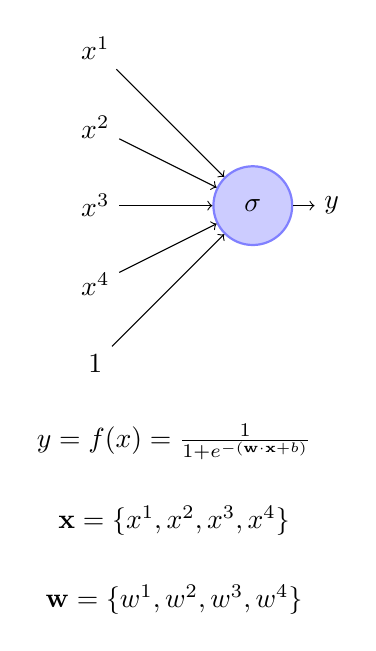
\begin{tikzpicture}
\node [neuron] (neuron0) at (1,4)  {$\sigma$} ;
\node (input0) at (-1,6)  {$x^1$};
\node (input1) at (-1,5)  {$x^2$};
\node (input2) at (-1,4)  {$x^3$};
\node (input3) at (-1,3)  {$x^4$};
\node (input4) at (-1,2)  {$1$};
\node (output0) at (2,4)  {$y$};
\node (formula) at (0,1) {$y = f(x)= \frac{1}{1+e^{-(\mathbf{w}\cdot \mathbf{x} + b)}}$};
\node (formula) at (0,0) {$\mathbf{x} = \{x^1, x^2, x^3, x^4\}$};
\node (formula) at (0,-1) {$\mathbf{w} = \{w^1, w^2, w^3, w^4\}$};
\draw [->] (input0) -- (neuron0);
\draw [->] (input1) -- (neuron0);
\draw [->] (input2) -- (neuron0);
\draw [->] (input3) -- (neuron0);
\draw [->] (input4) -- (neuron0);
\draw [->] (neuron0) -- (output0);
\end{tikzpicture}
